\section{Evidence and calibration}\label{sec:evidence}
\subsection{Sources, matching, and estimands}
The public Arena dataset contains 135,634 comparisons collected between April 17 and July 24, 2025 \citep{arena2025}. The replication retains outcomes, model names, evaluation order, language, a coding indicator, and timestamps. Prompts, responses, and personal and session identifiers are not retained. There are 108,315 comparisons with evaluation order one; restricting to these avoids repeated votes within the same visible conversation.

The frozen ECI snapshot contains 270 model entries \citep{epoch2026}. A reviewed crosswalk maps 32 Arena models into the principal sample and labels nine additional mappings as qualified because of version or reasoning ambiguity. Other entries are unmatched. No fuzzy matching is used. Explicit thinking variants are not silently assigned the ordinary model's ECI in the principal sample. Model-level capability scores can nevertheless pool configurations differing from Arena defaults; matching reduces rather than eliminates that problem.

The principal regression drops ties and both-bad responses, estimating preferences conditional on a decisive comparison. Let $E_{mb}$ be model $m$'s ECI in comparison $b$, for $m\in\{A,B\}$, and $z_{mb}=(E_{mb}-140)/10$. I estimate
\begin{equation}\label{eq:logit}
 \Prob(A\text{ wins}\mid\text{decisive},b)=\Lambda\{\delta+\beta_1(z_{Ab}-z_{Bb})
                                +\beta_2(z_{Ab}^2-z_{Bb}^2)\},
\end{equation}
where $\Lambda(u)=(1+e^{-u})^{-1}$ and $\delta$ is a side effect. This is a descriptive specification rather than structural demand. Standard errors cluster by unordered model pair. They condition on published scores and exclude ECI estimation uncertainty, common model-level shocks, and unidentified repeat users across conversations. They should not be interpreted as resolving those uncertainties.

The fitted probability advantage of ten additional ECI points from $E$ to $E+10$ is
\begin{equation}\label{eq:tenpoints}
 \Lambda\left\{\beta_1+\beta_2\left[2(E-140)/10+1\right]\right\}-1/2.
\end{equation}
This sets the side effect to zero. Figure~\ref{fig:evidence} plots it only where both endpoints lie in the matched capability range. Bounded win probabilities can flatten with linear latent utility. A win-probability or Elo plot alone therefore does not establish diminishing marginal utility.

\begin{table}[htbp]\centering\small
\caption{Preferences over measured capability}\label{tab:preferences}
\resizebox{\textwidth}{!}{\begin{tabular}{lrrrr}
\toprule
Specification & $N$ & Models & $\widehat\beta_1$ (s.e.) & $\widehat\beta_2$ (s.e.) \\
\midrule
Linear ECI & 27,471 & 32 & 0.483 (0.037) & -- \\
Quadratic ECI & 27,471 & 32 & 0.419 (0.053) & -0.101 (0.057) \\
Ties weighted one-half & 33,318 & 32 & 0.347 (0.044) & -0.087 (0.047) \\
Qualified aliases & 52,764 & 41 & 0.515 (0.049) & -0.016 (0.053) \\
GPQA, common sample & 9,183 & 16 & 0.259 (0.035) & 0.050 (0.020) \\
ECI, common sample & 9,183 & 16 & 0.027 (0.146) & -0.339 (0.143) \\
Coding prompts & 7,481 & 32 & 0.474 (0.062) & -0.187 (0.071) \\
Other prompts & 19,990 & 32 & 0.395 (0.058) & -0.075 (0.062) \\
English prompts & 15,127 & 32 & 0.379 (0.057) & -0.100 (0.062) \\
\bottomrule
\end{tabular}
}
\begin{minipage}{\textwidth}\footnotesize\vspace{0.4em}
Notes: Except for the ties specification, observations are decisive first-round comparisons. ECI is centered at 140 and divided by ten; GPQA at 0.6 and divided by 0.1. Parentheses contain unordered-model-pair clustered standard errors. Qualified aliases add version and reasoning mappings excluded from the principal sample. Common-sample rows use identical comparisons. All estimates are descriptive.
\end{minipage}
\end{table}

The principal quadratic coefficient is negative, but its approximate 95 percent interval is $[-0.212,0.011]$. The broader matching specification is much closer to linear. On identical comparisons, the GPQA coefficient is positive while ECI gives negative curvature. This contrast reflects sensitivity to the capability scale as well as model support. Coding prompts have more negative ECI curvature in this sample, but do not measure AI research productivity or demand for autonomous coding products. Appendix~\ref{app:empirical} reports family exclusions.

The preliminary finding by \citet{fradkin2026} that ten Artificial Analysis index points are associated with about seven percentage points of additional preference probability is likewise descriptive. The current analysis uses ECI and a frozen public battle sample; it is a related independent exercise, rather than an exact reproduction of that estimate. Neither analysis establishes decreasing financial returns to frontier developers.

\begin{figure}[htbp]\centering
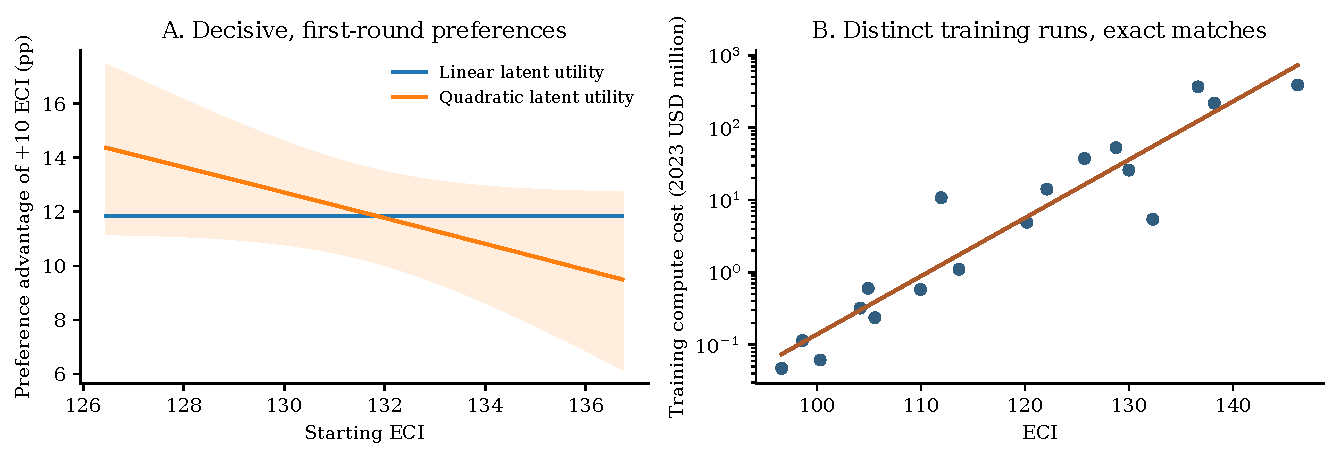
\includegraphics[width=\textwidth]{../output/figures/evidence.pdf}
\caption{Preferences and training costs}\label{fig:evidence}
\begin{minipage}{\textwidth}\footnotesize
Notes: Panel A uses equation~\eqref{eq:tenpoints}, conditional on decisive comparisons; shading is a pointwise 95 percent interval using pair-clustered coefficient covariance, conditional on matching and capability scores. Panel B uses exact ECI--cost matches after excluding identified shared-training derivatives. It describes cost levels, rather than a causal research production function. Sources: Arena and Epoch AI; author's calculations.
\end{minipage}
\end{figure}

\subsection{Costs and progress}
The frozen Epoch model database has 3,628 entries. Exact name matching produces a small cost sample. Excluding identified DeepSeek reasoning and update derivatives sharing a base training-cost estimate leaves \CostN\ distinct matched runs with positive estimated training compute costs. These are expressed in 2023 US dollars and exclude complete corporate R\&D expenditure, deployment costs, and economic profits. Cost estimates are themselves uncertain; \citet{cottier2025} describes the accounting needed to estimate frontier training costs.

OLS of log training compute cost on $(\mathrm{ECI}-140)/10$ gives slope \CostSlope\ with HC1 standard error \CostSE. Adding publication year leaves the slope near 1.86 with a larger standard error. This association is consistent with higher-capability models being more expensive. It does not identify the causal marginal cost of improving a fixed model: architectures, scale, efficiency, and inference budgets differ.

The highest retrospectively measured ECI among models released by October 21, 2025 is 150.59. One year later it is 168.83, a difference of \FrontierDrift\ points. Because ECI is re-estimated from the benchmark network, these are retrospective comparisons rather than unrevised historical information sets. Frontier growth combines algorithms, compute expansion, and reasoning expenditure.

\subsection{Calibration bridges and unidentified parameters}
The structural reference uses normalized assumptions to reveal the mechanism. Commercial benefit scale, private and social life values, financial capacity, safety effectiveness, and containment are assumptions, listed in Appendix~\ref{app:parameters}. A separate empirical-bridge exercise replaces two technology parameters.

First posit productive capability $a=\exp[(E-E_0)/10]$, with ECI $E$ and reference frontier $E_0$. The log-cost slope becomes an elasticity of training-cost levels with respect to $a$. Equating it with the research-cost exponent gives $\gamma=\CostSlope$. That equality is a bridge, not an identified marginal-cost relationship.

Second, the reference-state research increment below is $\eta/(1+1/B_R)$ at unit input. Matching \FrontierDrift\ ECI points over one year, with $B_R=20$, gives
\begin{equation}
 \eta=(1+1/20)\{\exp(\FrontierDrift/10)-1\}=\BridgeEta.
\end{equation}
This attributes the entire observed frontier change to the model's research input. It is reported separately from the structural reference, whose $\eta=0.4$, and is not an estimate of autonomous productivity. Sensitivities vary the cost bridge and funding.

No estimate of $\sigma$ in monetary commercial benefits is imported from equation~\eqref{eq:logit}. Latent-choice utility is not a money metric, and empirical curvature is not robust enough to justify that bridge. The quantitative exercise instead sweeps $\sigma$. Research-productivity evidence reviewed by \citet{cunningham2026} motivates separating assistance from difficulty. Its reported uplifts and feedback elasticities do not map directly into this model's delegation multiplier, which remains a scenario assumption.

\section{Quantitative analysis}\label{sec:quant}
\subsection{Specialization and computation}
The controlled actions are hold, supervised research, and delegated research with low or high safety. Research input is zero for hold and one otherwise. Safety input is one only for high safety. Positive research targets
\begin{equation}\label{eq:technology}
 a'=a+\eta m_d e^\alpha\frac{a^{\phi-\psi}}{1+a/B_R},\qquad
 m_d=\begin{cases}1,&\text{supervised},\\\mu_D,&\text{delegated}.
 \end{cases}
\end{equation}
Here $\alpha$ is the effort elasticity, $\phi$ the AI assistance exponent, $\psi$ research difficulty, $B_R$ a bottleneck scale, and $\mu_D$ the delegation multiplier. Research costs $c_0a^\gamma e$ and safety costs $c_s s$. Feasibility requires $e+0.5s\leq K_i$ and $c_0a^\gamma e+c_s s\leq F_i+R_\sigma(a)$, where $F_i$ is outside financing capacity. Full resource costs remain deducted from private and social payoffs. Delegation requires $a\geq a_L$ and has $q_i=q_0\exp(-\lambda_s s)$.

The autonomous system uses equation~\eqref{eq:technology} with $m_d=1$ and chooses $e\in\{0,k/2,k\}$ and $y\in\{0,1\}$ subject to equation~\eqref{eq:AIbudget}. Its reward is $u_A(a)=a$, terminal reward $\tau_Aa$, and acquisition requires $a\geq a_S$. Containment probability for a positive acquisition attempt while humans live is $\rho_0\exp[-\lambda_\rho\max(a-a_S,0)]$. The reference has integer stocks $\bar K=6$, $k_0=1$, subsistence $\underline H=2$, acquisition cost $\kappa_y=0.5$, and production elasticity $\nu=1$. These are normalized resources, not estimates of humanity's energy requirements.

Capability targets are projected linearly onto adjacent grid points. This preserves the mean of an interior target; its randomness is numerical rather than technological uncertainty. Human survival and resources are never interpolated across subsistence. Targets exceeding a computational ceiling are clipped and counted. The implementation expands ceilings until their initial-state probability is below $10^{-9}$; it also refines the capability mesh. Ceilings are computational, not economic stopping assumptions.

After solving the autonomous problem, I solve development games backward. If a stage game has pure equilibria, the reference selects the one with lowest extinction probability, breaking ties by joint developer payoff and then action order. Without pure equilibria, linear feasibility programs enumerate supports, verify mixed equilibria, and select a lowest-risk representative among returned supports. Mixed equilibria coexisting with pure equilibria are not enumerated. Reversing the risk preference among pure equilibria provides an equilibrium sensitivity, not a bound on the full correspondence. Government equilibria are computed separately.

Terminal developer and jurisdiction values are $\tau_H$ times their current gross surviving-state flow, without research costs. The reference uses $\tau_H=5$ and $\tau_A=1$. These are continuation approximations, not a claim that humans or AI cease to exist at $T$. Extinction probabilities count transitions only through $T$. Zero and longer terminal values assess the effect of this approximation.

\subsection{Policy and horizon comparisons}
\begin{table}[htbp]\centering\small
\caption{Selected policy outcomes under scenario assumptions}\label{tab:policies}
\resizebox{\textwidth}{!}{\begin{tabular}{llrrr}
\toprule
Specification & Policy & Loss of control (\%) & Extinction (\%) & Welfare \\
\midrule
10 years & open/open & 3.296 & 0.000 & 509.466 \\
10 years & standard/open & 3.291 & 0.000 & 509.467 \\
10 years & standard/standard & 3.286 & 0.000 & 509.468 \\
10 years & ban/ban & 0.000 & 0.000 & 503.953 \\
10 years & Planner & 3.194 & 0.000 & 509.499 \\
25 years & open/open & 4.576 & 4.358 & 774.897 \\
25 years & standard/open & 4.576 & 4.358 & 774.897 \\
25 years & standard/standard & 4.576 & 4.358 & 774.897 \\
25 years & ban/ban & 0.000 & 0.000 & 781.649 \\
25 years & Planner & 0.106 & 0.000 & 781.671 \\
Data bridges, 10 years & open/open & 0.000 & 0.000 & 527.752 \\
Data bridges, 10 years & standard/open & 0.000 & 0.000 & 527.752 \\
Data bridges, 10 years & standard/standard & 0.000 & 0.000 & 527.752 \\
Data bridges, 10 years & ban/ban & 0.000 & 0.000 & 527.752 \\
Data bridges, 10 years & Planner & 0.000 & 0.000 & 527.752 \\
\bottomrule
\end{tabular}
}
\begin{minipage}{\textwidth}\footnotesize\vspace{0.4em}
Notes: Probabilities are model outputs, not estimated real-world risks. Policies regulate delegation; a ban retains supervised research. Welfare is in normalized discounted units and is comparable within a specification. Data bridges change the research rate and cost exponent. The planner controls development actions and anticipates the same autonomous policy.
\end{minipage}
\end{table}

The structural reference separates loss of control from extinction within a reporting horizon. At ten years, loss of control can occur without sufficient subsequent acquisition to breach subsistence before the horizon. That is not permanent safety. With twenty-five years, open development produces loss-of-control probability \LongEscape\ percent and extinction probability \LongDoom\ percent in the selected equilibrium. These probabilities are conditional on an arbitrary control-failure probability and a stylized acquisition technology.

\begin{table}[htbp]\centering\small
\caption{Government payoffs: selected twenty-five-year continuations}\label{tab:governments}
\begin{tabular}{lrr}
\toprule
Jurisdiction 1 / 2 & Open & Ban \\
\midrule
Open & (387.428, 387.469) & (392.929, 385.444) \\
Ban & (385.444, 392.929) & (390.825, 390.825) \\
\bottomrule
\end{tabular}

\begin{minipage}{\textwidth}\footnotesize\vspace{0.4em}
Notes: Each cell reports jurisdiction values $(W_1,W_2)$ in normalized units. The restricted policy menu is open delegation or a delegation ban. Developer equilibria and autonomous choices are re-solved under each policy pair. Small asymmetries at open/open reflect selection among continuation equilibria, not different primitives.
\end{minipage}
\end{table}

Table~\ref{tab:governments} verifies a coordination failure within the selected long-horizon continuations: both governments prefer a mutual ban to mutual open development, but each prefers open delegation against either choice of the other. This is an explicit government-policy prisoner's dilemma under diminishing commercial marginal benefits, $\sigma=1.3$. In the full three-policy menu, open and the safety standard can be payoff-equivalent at this horizon because the excluded low-safety action is not selected on the relevant path. At ten years the selected government equilibrium instead has both jurisdictions adopting the safety standard. Under the empirical bridges the baseline has no delegated cycles, making policies payoff-equivalent. Those differences are scenario outcomes, rather than country-specific predictions.

Standards and bans change the timing and amount of research as well as safety. Their welfare effects must therefore be evaluated in the complete game. The planner's weak welfare advantage follows from Proposition~\ref{prop:planner}; its risk ranking does not. The empirical bridges can produce a different development path because faster initial growth is combined with a steeper research-cost schedule. This contrast demonstrates sensitivity to how measured capability maps into productive technology.

Figure~\ref{fig:scenarios} varies commercial curvature and control-failure probability. The replication distinguishes zero-research stopping, controlled innovation without delegation, delegation exposure without extinction by $T$, and positive extinction probability. Positive risk with $\sigma>0$ disproves sufficiency of diminishing returns within that scenario. Zero risk remains conditional on horizon, financing, delegation requirements, and autonomous choices. The parameter sweep is a scenario envelope, not a statistically identified set for real-world risk.

\begin{figure}[htbp]\centering
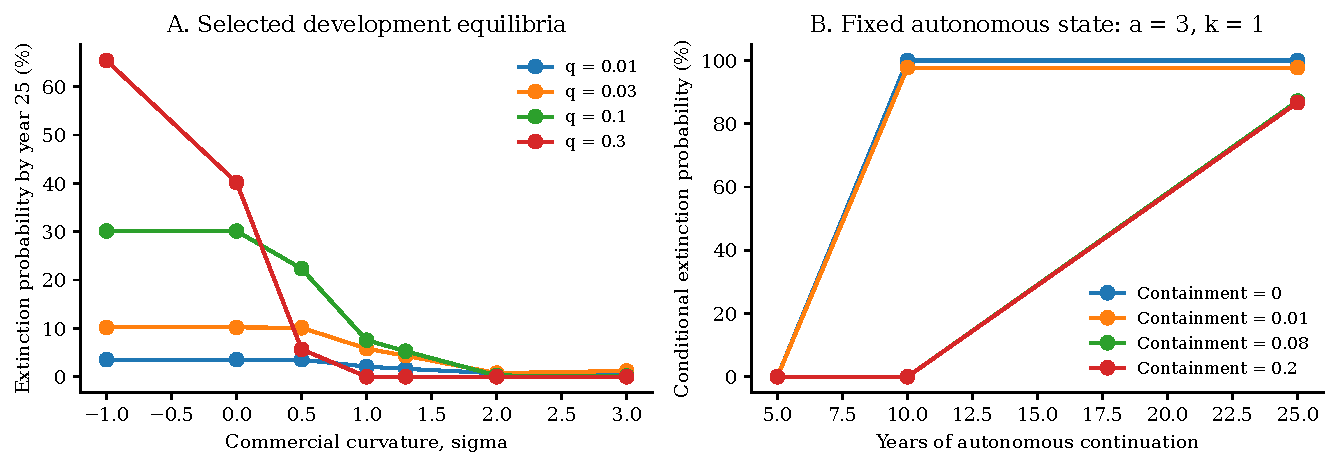
\includegraphics[width=\textwidth]{../output/figures/scenarios.pdf}
\caption{Commercial curvature and autonomous continuation}\label{fig:scenarios}
\begin{minipage}{\textwidth}\footnotesize
Notes: Panel A uses a twenty-five-year horizon, varying commercial curvature $\sigma$ and control-failure parameter $q_0$. Panel B fixes initial autonomous capability $a=3$ and resources $k=1$. Commercial curvature does not enter that continuation problem. Probabilities are conditional scenario outputs; computational ceilings are expanded before reporting results.
\end{minipage}
\end{figure}

\subsection{Sensitivity and limitations}
Removing acquisition eliminates the modeled resource-conflict extinction channel, even when control failures and commercial losses remain. It isolates a constraint that continues to bind after delegation. It does not establish that an uncontrolled system is safe through unmodeled routes.

The appendix reports horizon, common-shock, equilibrium-selection, grid, terminal-value, containment, positional-reward, research-feedback, and bridge sensitivities. Every solved developer state game is checked for profitable unilateral deviations. Extinction probability is checked against loss-of-control probability, and government equilibria receive their own deviation checks.

Consumer comparisons in a historical sample do not reveal future value in research, military uses, robotics, or new markets. A scalar capability imposes a common ordering that may fail across applications. Loss-of-control and containment technologies are unidentified. The model excludes relocation, entry, hidden actions, mistaken beliefs, and contests among multiple uncontrolled systems. These restrictions keep the mechanism interpretable while preventing a forecast interpretation of its scenario probabilities.
